% !TEX program = xelatex
% Question 1 full technical report. Build from this folder:  xelatex Q1_report.tex  (twice)   or   latexmk -xelatex Q1_report.tex
% Tables are generated from outputs/results/*.json by make_tables.py -> tables.tex. Figures come from ../outputs/figures/.
\documentclass[10pt,a4paper]{article}

\usepackage[margin=2.0cm]{geometry}
\usepackage{fontspec}
\usepackage{amsmath,amssymb}
\usepackage{graphicx}
\usepackage{booktabs}
\usepackage{array}
\usepackage{xcolor}
\usepackage{microtype}
\usepackage{float}
\usepackage[font=small,labelfont=bf,skip=4pt]{caption}
\usepackage{enumitem}
\usepackage{fancyhdr}
\usepackage{needspace}
\usepackage{etoolbox}
\pretocmd{\section}{\Needspace*{9\baselineskip}}{}{}
\usepackage{titlesec}
\usepackage[colorlinks=true,linkcolor=blue!40!black,urlcolor=blue!50!black]{hyperref}

\IfFontExistsTF{Noto Serif Devanagari}{\newfontfamily\hindifont[Script=Devanagari]{Noto Serif Devanagari}}{%
\IfFontExistsTF{Noto Sans Devanagari}{\newfontfamily\hindifont[Script=Devanagari]{Noto Sans Devanagari}}{%
\IfFontExistsTF{FreeSerif}{\newfontfamily\hindifont[Script=Devanagari]{FreeSerif}}{%
\newfontfamily\hindifont[Script=Devanagari]{Latin Modern Roman}}}}
\DeclareRobustCommand{\hi}[1]{{\hindifont #1}}

\definecolor{accent}{HTML}{1F4E79}
\titleformat{\section}{\large\bfseries\color{accent}}{\thesection}{0.6em}{}[\vspace{-0.4em}{\color{accent}\titlerule}]
\titleformat{\subsection}{\normalsize\bfseries\color{accent}}{\thesubsection}{0.6em}{}
\titlespacing*{\section}{0pt}{12pt}{6pt}
\titlespacing*{\subsection}{0pt}{8pt}{3pt}

\makeatletter
\def\maxwidth{\ifdim\Gin@nat@width>\linewidth\linewidth\else\Gin@nat@width\fi}
\makeatother
\setkeys{Gin}{width=\maxwidth,keepaspectratio}
\setlist{itemsep=2pt,topsep=3pt,parsep=0pt}
\setlength{\parskip}{4pt}
\setlength{\parindent}{0pt}
\setlength{\emergencystretch}{3em}
\renewcommand{\arraystretch}{1.15}
\setlength{\tabcolsep}{5pt}
\pagestyle{fancy}\fancyhf{}
\fancyhead[L]{\small DSL 504 NLP, Group Assignment 2}\fancyhead[R]{\small Question 1: Attention-based NMT}
\fancyfoot[C]{\small\thepage}
\renewcommand{\headrulewidth}{0.3pt}

% ---- Metrics
\newcommand{\tabMetrics}{
\begin{tabular}{lrr}\toprule
Test metric (2,393 sentences) & A: baseline & B: attention \\ \midrule
BLEU (corpus, sacreBLEU 13a) & 0.55 & \textbf{2.34} \\
chrF & 12.27 & \textbf{17.91} \\
chrF++ & 11.54 & \textbf{17.37} \\
TER (lower is better) & 104.03 & \textbf{99.12} \\
BLEU 1-gram precision & 15.89 & \textbf{23.98} \\
BLEU 2-gram precision & 2.17 & \textbf{5.33} \\
BLEU 3-gram precision & 0.19 & \textbf{1.13} \\
BLEU 4-gram precision & 0.01 & \textbf{0.21} \\
Brevity penalty & 1.000 & 1.000 \\
Length ratio (hyp/ref) & 1.033 & 1.087 \\
Hypothesis tokens / reference tokens & 58,459 / 56,583 & 61,516 / 56,583 \\
\bottomrule\end{tabular}}
% ---- Loss
\newcommand{\tabLoss}{
\begin{tabular}{lrr}\toprule
Training / validation / test & A: baseline & B: attention \\ \midrule
Best epoch (lowest val. loss) & 4 & 4 \\
Train loss at best epoch & 4.542 & 3.633 \\
Validation loss & 5.180 & 4.754 \\
Test loss & 5.078 & 4.665 \\
Test perplexity & 160.4 & 106.2 \\
Train token accuracy at best epoch & 0.248 & 0.325 \\
Validation token accuracy & 0.249 & 0.298 \\
Test token accuracy & 0.243 & 0.290 \\
Parameters & 38,334,930 & 71,896,274 \\
Seconds per epoch & 48 & 222 \\
\bottomrule\end{tabular}}
% ---- History
\newcommand{\tabHistory}{
\begin{tabular}{r|rrrr|rrrr}\toprule
Epoch & \multicolumn{4}{c}{A: baseline} & \multicolumn{4}{c}{B: attention} \\ & train loss & val loss & train acc & val acc & train loss & val loss & train acc & val acc \\ \midrule
1 & 6.200 & 5.568 & 0.136 & 0.208 & 5.862 & 5.331 & 0.167 & 0.234 \\
2 & 5.268 & 5.323 & 0.201 & 0.231 & 4.795 & 4.977 & 0.245 & 0.274 \\
3 & 4.853 & 5.245 & 0.228 & 0.243 & 4.149 & 4.813 & 0.288 & 0.287 \\
\textbf{4} & \textbf{4.542} & \textbf{5.180} & \textbf{0.248} & \textbf{0.249} & \textbf{3.633} & \textbf{4.754} & \textbf{0.325} & \textbf{0.298} \\
5 & 4.291 & 5.184 & 0.264 & 0.252 & 3.216 & 4.760 & 0.364 & 0.298 \\
6 & 4.076 & 5.200 & 0.278 & 0.255 & 2.895 & 4.780 & 0.400 & 0.303 \\
7 & 3.887 & 5.212 & 0.292 & 0.255 & 2.647 & 4.814 & 0.432 & 0.307 \\
8 & 3.721 & 5.242 & 0.305 & 0.261 & 2.458 & 4.850 & 0.459 & 0.309 \\
\bottomrule\end{tabular}}
% ---- BucketA
\newcommand{\tabBucketA}{
\begin{tabular}{lrrrrrrrrrr}\toprule
EN length & n & BLEU & p1 & p2 & p3 & p4 & BP & ratio & chrF & TER \\ \midrule
1-5 & 13 & 3.07 & 20.5 & 5.7 & 1.8 & 1.1 & 0.786 & 0.806 & 7.61 & 91.3 \\
6-10 & 282 & 0.41 & 14.2 & 2.1 & 0.0 & 0.0 & 0.969 & 0.970 & 8.96 & 102.2 \\
11-15 & 481 & 0.48 & 14.1 & 2.3 & 0.1 & 0.0 & 1.000 & 1.119 & 10.74 & 108.5 \\
16+ & 1,617 & 0.57 & 16.3 & 2.2 & 0.2 & 0.0 & 1.000 & 1.024 & 12.73 & 103.5 \\
\midrule all & 2,393 & 0.55 & 15.9 & 2.2 & 0.2 & 0.0 & 1.000 & 1.033 & 12.27 & 104.0 \\
\bottomrule\end{tabular}}
% ---- BucketB
\newcommand{\tabBucketB}{
\begin{tabular}{lrrrrrrrrrr}\toprule
EN length & n & BLEU & p1 & p2 & p3 & p4 & BP & ratio & chrF & TER \\ \midrule
1-5 & 13 & 2.13 & 26.7 & 4.8 & 1.0 & 0.7 & 0.688 & 0.728 & 12.77 & 84.5 \\
6-10 & 282 & 2.73 & 27.7 & 6.9 & 1.5 & 0.3 & 0.931 & 0.933 & 16.03 & 88.9 \\
11-15 & 481 & 2.74 & 25.9 & 6.3 & 1.3 & 0.3 & 1.000 & 1.034 & 17.13 & 94.0 \\
16+ & 1,617 & 2.26 & 23.5 & 5.1 & 1.1 & 0.2 & 1.000 & 1.106 & 18.16 & 100.6 \\
\midrule all & 2,393 & 2.34 & 24.0 & 5.3 & 1.1 & 0.2 & 1.000 & 1.087 & 17.91 & 99.1 \\
\bottomrule\end{tabular}}
% ---- Compare
\newcommand{\tabCompare}{
\begin{tabular}{lrrrrrrrr}\toprule
EN length & n & BLEU A & BLEU B & B/A & chrF A & chrF B & repeats A & repeats B \\ \midrule
1-5 & 13 & 3.07 & 2.13 & 0.7$\times$ & 7.61 & 12.77 & 0.0\% & 15.4\% \\
6-10 & 282 & 0.41 & 2.73 & 6.8$\times$ & 8.96 & 16.03 & 0.4\% & 5.7\% \\
11-15 & 481 & 0.48 & 2.74 & 5.7$\times$ & 10.74 & 17.13 & 0.2\% & 8.7\% \\
16+ & 1,617 & 0.57 & 2.26 & 4.0$\times$ & 12.73 & 18.16 & 0.5\% & 17.6\% \\
\bottomrule\end{tabular}}
% ---- Recall
\newcommand{\tabRecall}{
\begin{tabular}{lrrrr}\toprule
Unigram recall, 16+ tokens & Q1 (first) & Q2 & Q3 & Q4 (last) \\ \midrule
A: baseline & 0.165 & 0.154 & 0.130 & 0.223 \\
B: attention & 0.275 & 0.252 & 0.230 & 0.284 \\
\bottomrule\end{tabular}}
% ---- Attn
\newcommand{\tabAttn}{
\begin{tabular}{lr}\toprule
Attention statistic & Value \\ \midrule
Test sentences analysed & 2,393 \\
Mean peak attention weight & 0.277 \\
Mean attention entropy (nats) & 2.325 \\
Steps whose peak stays or moves forward & 85.3\% \\
Mean deviation from the diagonal (relative) & 0.218 \\
Steps with multi-word attention & 20.6\% \\
Attention mass on \textless{}sos\textgreater{}/\textless{}eos\textgreater{} & 1.03\% \\
Generated tokens that occur in the reference & 39.2\% \\
Mean peak weight, token in reference & 0.2769 \\
Mean peak weight, token not in reference & 0.2768 \\
Wrong tokens generated with peak weight $>0.7$ & 1.52\% \\
\bottomrule\end{tabular}}
% ---- Data
\newcommand{\tabData}{
\begin{tabular}{lr}\toprule
Data statistic & Value \\ \midrule
Raw training pairs in IITB corpus & 1,659,083 \\
Training pairs used (random draw, seed 42) & 50,000 \\
Development pairs / test pairs (official, cleaned) & 514 / 2,393 \\
English vocabulary size & 21,433 \\
Hindi vocabulary size & 24,274 \\
Maximum English / Hindi sentence length (tokens) & 50 / 50 \\
Mean length, training (English / Hindi) & 17.7 / 18.4 \\
OOV rate, dev (English / Hindi) & 6.0\% / 8.6\% \\
OOV rate, test (English / Hindi) & 8.4\% / 8.0\% \\
\bottomrule\end{tabular}}
\newcommand{\errorcase}[1]{%
\ifcase#1\or
\begin{minipage}{\linewidth}\small
\textbf{Case 1} (test sentence \#2171; sentence chrF: baseline 10.7, attention 23.2; error type: \emph{long-distance dependency; wrong attention focus; OOV names; repetition})\\[2pt]
\begin{tabular}{@{}l p{0.86\linewidth}@{}}
EN & " i'm not sure when he sleeps , " said katie o'malley , a second-year medical student from drexel university in philadelphia and volunteer with bwelle's group . \\
Ref & \hi{फिलाडेल्फिया में ड्रेक्सेल विश्वविद्यालय की द्वितीय वर्ष की चिकित्सा विद्यार्थी और वेल के समूह में स्वयंसेवी} , \hi{कैटी ओ}'\hi{मैली ने कहा} , " \hi{मुझे नहीं पता कि वे सोते कब हैं ।} " \\
A & ( \hi{ऐ रसूल} ) \hi{तुम कह दो कि ख़ुदा ने अपने परवरदिगार की तरफ से इन्कार किया और} ( \hi{ऐ रसूल} ) \hi{तुम कह दो कि तुम लोग तो बस अपने परवरदिगार की राह से इन्कार करो} \\
B & " \hi{जब उन्होंने कहा कि जब उन्होंने कहा कि} " \hi{आचार्य} , " \hi{आचार्य} , \hi{श्री राम नाथ कोविन्द से पूर्व मुख्यमंत्री विश्वविद्यालय के साथ} , \hi{एक और अन्य लेखकों के साथ एक अन्य लेखकों और अन्य महानुभावों के साथ} ‘ ‘ \hi{द रिट्रीट} ’ ’ \hi{नामक हैं ।} \\
\end{tabular}\\[2pt]
\textit{Reading the heatmap:} Attention starts sensibly (the quoted clause), then sits on one source column ('university') for about 12 consecutive steps while the decoder invents '\hi{आचार्य श्री राम नाथ कोविन्द}'. Later it loops '\hi{एक अन्य लेखकों के साथ}' while attending 'medical student'. The heatmap shows the stuck column, which explains the drift. \textit{Useful as explanation?} yes, it shows where the model got stuck.
\end{minipage}
\or
\begin{minipage}{\linewidth}\small
\textbf{Case 2} (test sentence \#799; sentence chrF: baseline 12.0, attention 23.8; error type: \emph{OOV (bcci, mca); extra/repeated words})\\[2pt]
\begin{tabular}{@{}l p{0.86\linewidth}@{}}
EN & afterwards , there would be a joint presentation by the bcci and the mca . \\
Ref & \hi{इसके बाद बीसीसीआइ और एमसीए द्वारा संयुक्त प्रस्तुतिकरण होगा ।} \\
A & \hi{एक बार फिर से एक दूसरे के लिए एक दूसरे से एक दूसरे के साथ एक दूसरे से बाहर हो गया है ।} \\
B & \hi{इसके अतिरिक़्त} , \hi{और और इस द्वारा द्वारा एक ही एक ही एक ही होगा ।} \\
\end{tabular}\\[2pt]
\textit{Reading the heatmap:} The first words align diagonally (afterwards -\textgreater{} \hi{इसके अतिरिक्त}). Attention then lands on 'joint presentation' (correct focus) but the decoder emits '\hi{एक ही एक ही एक ही}' instead of '\hi{संयुक्त प्रस्तुतिकरण}'. The two acronyms are unknown source words, so '\hi{और इस द्वारा द्वारा}' is filler. \textit{Useful as explanation?} partly: focus is right, output is wrong.
\end{minipage}
\or
\begin{minipage}{\linewidth}\small
\textbf{Case 3} (test sentence \#1127; sentence chrF: baseline 8.1, attention 31.9; error type: \emph{OOV (tassie); missing word (\$325m); wrong word})\\[2pt]
\begin{tabular}{@{}l p{0.86\linewidth}@{}}
EN & \$325m rescue package for tassie health \\
Ref & \hi{टैजी के स्वास्थ्य के लिए} 325 \hi{मिलियन डॉलर का बचाव पैकेज} \\
A & \hi{एक नया स्रोत जिसमें एक नया} \\
B & \hi{स्वास्थ्य के लिए माइक्रोसॉफ़्ट अनुरोध} \\
\end{tabular}\\[2pt]
\textit{Reading the heatmap:} 'tassie health' correctly drives '\hi{स्वास्थ्य के लिए}'. 'rescue package' is attended with weight about 0.45 but translated as '\hi{माइक्रोसॉफ़्ट अनुरोध}' (a hallucination for '\hi{बचाव पैकेज}'). The number is dropped and the output ends early. \textit{Useful as explanation?} partly: correct source words attended, wrong target words.
\end{minipage}
\or
\begin{minipage}{\linewidth}\small
\textbf{Case 4} (test sentence \#2031; sentence chrF: baseline 10.9, attention 38.5; error type: \emph{wrong word (\hi{विदेशों} missing); repetition; word order})\\[2pt]
\begin{tabular}{@{}l p{0.86\linewidth}@{}}
EN & his name became known not only in the country , but also abroad . \\
Ref & \hi{उनका नाम देश ही नहीं बल्कि विदेशों में भी प्रसिद्ध हुआ ।} \\
A & \hi{वह अपने पिता के साथ एक दूसरे से बाहर नहीं थे ।} \\
B & \hi{उनका नाम केवल देश में ही नहीं बल्कि बल्कि भी भी भी थीं ।} \\
\end{tabular}\\[2pt]
\textit{Reading the heatmap:} Best diagonal alignment of the eight. 'abroad' receives the highest weight (about 0.65) for three steps in a row, yet the model emits '\hi{भी भी भी}' instead of '\hi{विदेशों में}'. A very high weight does not mean a correct word. '\hi{बल्कि}' is also generated twice. \textit{Useful as explanation?} yes for locating the failure, no as a guarantee of correctness.
\end{minipage}
\or
\begin{minipage}{\linewidth}\small
\textbf{Case 5} (test sentence \#2278; sentence chrF: baseline 15.1, attention 22.9; error type: \emph{OOV names missing; wrong word; extra words})\\[2pt]
\begin{tabular}{@{}l p{0.86\linewidth}@{}}
EN & according to amarnath upadhyaya , secretary of ada , a proposal concerning this matter has been sent to the government . \\
Ref & \hi{एडीए के सचिव अमरनाथ उपाध्याय के मुताबिक इस बाबत शासन को प्रस्ताव भेजा जा चुका है ।} \\
A & \hi{इस प्रकार के दौरान} , \hi{इस क्षेत्र में एक बड़ी संख्या में एक बड़ी भूमिका है ।} \\
B & \hi{इस बात के अनुसार} , \hi{श्री एक समिति के अनुसार} , \hi{इस अध्याय को इस सरकार को इस बैठक में भेजा गया है ।} \\
\end{tabular}\\[2pt]
\textit{Reading the heatmap:} Mostly monotone alignment. The OOV names (amarnath upadhyaya, ada) are replaced by generic words ('\hi{श्री एक समिति के अनुसार}'). The ending is good: 'sent' -\textgreater{} '\hi{भेजा गया है}' with weight about 0.45 and 'government' -\textgreater{} '\hi{सरकार}', but '\hi{बैठक में}' (meeting) is hallucinated while attending 'sent'. \textit{Useful as explanation?} yes.
\end{minipage}
\or
\begin{minipage}{\linewidth}\small
\textbf{Case 6} (test sentence \#2388; sentence chrF: baseline 11.9, attention 23.7; error type: \emph{OOV names missing; wrong word (semantic neighbour)})\\[2pt]
\begin{tabular}{@{}l p{0.86\linewidth}@{}}
EN & it is noteworthy that both nita and isha are professional , classical dancers . \\
Ref & \hi{गौरतलब है कि नीता और ईशा दोनों ही प्रोफेशनल क्लासिकल डांसर है ।} \\
A & \hi{यह एक बड़ी बात है कि यह एक बड़ी बात है कि एक दूसरे के लिए एक बड़ी समस्या है ।} \\
B & \hi{यह जानकर प्रसन्नता है कि दोनों और दोनों ही शैली में हैं} , \hi{और शास्त्रीय संगीत हैं ।} \\
\end{tabular}\\[2pt]
\textit{Reading the heatmap:} Near-perfect diagonal: 'both' -\textgreater{} '\hi{दोनों}' (weight about 0.85), 'classical' -\textgreater{} '\hi{शास्त्रीय}'. The names nita and isha are unknown and dropped. 'dancers' becomes '\hi{संगीत}' (music) and 'professional' becomes '\hi{शैली}' (style), so the alignment looks right while two words are wrong. \textit{Useful as explanation?} misleading: the heatmap looks like a good translation.
\end{minipage}
\or
\begin{minipage}{\linewidth}\small
\textbf{Case 7} (test sentence \#800; sentence chrF: baseline 10.0, attention 31.4; error type: \emph{repetition; missing content words; long-distance dependency})\\[2pt]
\begin{tabular}{@{}l p{0.86\linewidth}@{}}
EN & besides that , a special coin would be used for the coin toss that would be kept by the mca . \\
Ref & \hi{इसके अलावा टॉस के लिए एक विशेष सिक्के का इस्तेमाल किया जाएगा जिसे एमसीए संभालकर रखेगा ।} \\
A & \hi{यह एक बड़ी बात है कि यह एक बड़ी बात है जो एक दूसरे के साथ एक दूसरे से अधिक है ।} \\
B & \hi{इसके अलावा} , \hi{एक विशेष रूप से एक विशेष रूप से प्रयोग किया जाएगा} , \hi{जो कि वह इस प्रकार के द्वारा किया जाएगा कि वह द्वारा स्वंय के द्वारा किया जाएगा} . \\
\end{tabular}\\[2pt]
\textit{Reading the heatmap:} The first half is a clean diagonal ('besides that, a special coin' -\textgreater{} '\hi{इसके अलावा एक विशेष}'). From 'would be used' on, attention spreads over several source words and the decoder repeats '\hi{किया जाएगा} / \hi{द्वारा}' three times. 'coin toss' (\hi{टॉस}) and 'mca' are never translated. \textit{Useful as explanation?} yes: the diagonal breaks where the output goes wrong.
\end{minipage}
\or
\begin{minipage}{\linewidth}\small
\textbf{Case 8} (test sentence \#1568; sentence chrF: baseline 20.1, attention 23.3; error type: \emph{long-distance dependency; wrong attention focus (punctuation); repetition; word order})\\[2pt]
\begin{tabular}{@{}l p{0.86\linewidth}@{}}
EN & " our ongoing inquiry into this matter continues and we are co-operating fully with the fca and our other regulators , " the bank said two weeks ago . \\
Ref & \hi{दो सप्ताह पहले बैंक ने कहा था कि} , " \hi{इस मामले में हमारी जांच जारी है} , \hi{तथा हम} FCA \hi{और अन्य विनियामकों के साथ पूर्ण सहयोग कर रहे हैं ।} " \\
A & \hi{मैं इस अवसर पर आपके लिए बधाई देता हूं कि हमारे देश में हमारे देश के बीच द्विपक्षीय संबंधों में हमारे देश में हमारे देश में हमारे देश में सहयोग की है ।} \\
B & \hi{हमारे इस क्षेत्र में हम इस तरह के साथ ही हम एक दूसरे और अन्य शब्दों के साथ बातचीत की हैं और हम दोनों के दो शब्दों में} ‘ ‘ \hi{द} ’ ’ ’ ’ \hi{के साथ ही हम दोनों को भी कहा जाता है ।} \\
\end{tabular}\\[2pt]
\textit{Reading the heatmap:} A 30-token sentence whose clause 'the bank said two weeks ago' belongs at the front of the Hindi. The model drifts: in the last ten steps attention is anchored on the closing quote mark and the output degenerates into punctuation ('‘ ‘ \hi{द} ’ ’ ’ ’'). 'two weeks' becomes '\hi{दो शब्दों}' (two words). \textit{Useful as explanation?} yes: attention on punctuation signals the collapse.
\end{minipage}
\fi}

\newcommand{\code}[1]{\texttt{#1}}
\newcommand{\sos}{\texttt{<sos>}}
\newcommand{\eos}{\texttt{<eos>}}
\newcommand{\unk}{\texttt{<unk>}}

\begin{document}

\begin{center}
{\LARGE\bfseries\color{accent} Attention-Based English-to-Hindi\\[2pt] Neural Machine Translation}\\[6pt]
{\large Question 1 report | DSL 504 Natural Language Processing, Group Assignment 2}\\[3pt]
Rishi Kharya \quad|\quad IIT Bombay English-Hindi corpus \quad|\quad November 2026
\end{center}
\vspace{2pt}

\begin{center}\fbox{\parbox{0.94\linewidth}{\small
\textbf{Summary.} We built an English-to-Hindi translator with a 2-layer bidirectional LSTM encoder and a 2-layer LSTM decoder,
first without attention (Model A, 38.3M parameters) and then with our own Bahdanau attention (Model B, 71.9M parameters).
Both were trained on 50,000 IITB sentence pairs under the same conditions and evaluated on the 2,393-sentence official test set.
Attention improves \textbf{every} measure: BLEU \textbf{0.55 $\rightarrow$ 2.34}, chrF \textbf{12.27 $\rightarrow$ 17.91},
chrF++ 11.54 $\rightarrow$ 17.37, TER 104.0 $\rightarrow$ 99.1, test loss 5.078 $\rightarrow$ 4.665 (perplexity 160.4 $\rightarrow$ 106.2),
and test token accuracy 0.243 $\rightarrow$ 0.290. Absolute BLEU is low for both models (small data, word-level vocabulary, mixed-domain
corpus), so conclusions are about the \emph{difference} between A and B, from one seed. The attention heatmaps are mostly diagonal-forward,
sharp on content words and diffuse on function words, but a high attention weight does \emph{not} indicate a correct word.}}\end{center}

\tableofcontents

%--------------------------------------------------------------------------------------------------------------
\section{Task and approach}
The brief asks for an English-to-Hindi NMT system built as an LSTM encoder-decoder, first without and then with attention, with
(i) preprocessing statistics, (ii) a baseline and an analysis of its limitation on long sentences, (iii) our own attention
implementation whose weights can be inspected, (iv) a controlled comparison with training/validation curves, (v) attention
heatmaps, (vi) an attention-based error analysis of at least five sentences, (vii) performance by sentence length
(1--5, 6--10, 11--15, 16+ tokens), and (viii) a final comparative analysis. Sections 2 to 10 follow that order; section 11 lists
where every number in this report is stored.

%--------------------------------------------------------------------------------------------------------------
\section{Data preparation}
\textbf{Corpus.} IIT Bombay English-Hindi parallel corpus (HuggingFace \code{cfilt/iitb-english-hindi}), using the official
train / development / test split. Training data were used for fitting, the development set for model selection (early stopping on
validation loss), and the test set only for the final evaluation.

\begin{table}[H]\centering\tabData\caption{Data statistics (from \code{outputs/results/attention\_seed42/data\_stats.json}).}\end{table}

\textbf{Pipeline.} (1) Unicode NFC normalisation; English is lower-cased. (2) Punctuation, including the Hindi danda
\hi{।}, is split into its own token, then whitespace tokenisation. (3) \sos{} and \eos{} are added to every sentence, e.g.\
\texttt{<sos> i am going to school . <eos>} and \texttt{<sos>} \hi{मैं स्कूल जा रहा हूँ ।} \texttt{<eos>}. (4) Source and target vocabularies are
built from the training pairs only (\code{min\_freq=2}; ids \code{<pad>=0, <unk>=1, <sos>=2, <eos>=3}); everything rarer is \unk{}.
(5) Sentences are converted to ids and right-padded per batch.

\textbf{Malformed pairs removed.} Empty sides; either side outside 1--50 tokens; no Latin letter on the English side or no Devanagari
on the Hindi side; and, for training only, a length ratio above 3. Training pairs must also have at least 5 English tokens: the corpus
contains many one-word interface strings, while the dev and test sets are news-style sentences. Dev and test are not otherwise filtered.

\textbf{The test set is dominated by long sentences.} 1,617 of the 2,393 test sentences (67.6\%) have 16 or more English tokens, 481 have
11--15, 282 have 6--10, and only 13 have 1--5. Results for the 1--5 bucket are therefore not reliable. The test OOV rate is 8.4\% (English)
and 8.0\% (Hindi), which caps what a word-level model can reach.

%--------------------------------------------------------------------------------------------------------------
\section{Models}
Both models share one encoder: embedding (256) $\rightarrow$ 2-layer \textbf{bidirectional LSTM} (hidden 512, dropout 0.3) run on packed
sequences so that padding never enters the recurrence.

\textbf{Model A, baseline (no attention).} The encoder's final hidden and cell states (the two directions are merged and projected)
initialise a 2-layer LSTM decoder. This single fixed-size vector is the \emph{only} information the decoder receives about the source.
The decoder output goes through a dense layer and softmax over the Hindi vocabulary.

\textbf{Model B, attention.} All encoder states $h_1,\dots,h_n$ are kept. At every decoding step $t$ the decoder state $s_{t-1}$ is scored
against each $h_i$ with additive (Bahdanau) attention,
\[
e_{t,i} = v^{\top}\tanh(W_s s_{t-1} + W_h h_i),\qquad
\alpha_{t,i} = \frac{\exp(e_{t,i})}{\sum_j \exp(e_{t,j})},\qquad
c_t = \sum_i \alpha_{t,i}\, h_i ,
\]
with padded source positions masked out before the softmax. The context $c_t$ is concatenated to the decoder input and to the features
before the output softmax. This is our own implementation (\code{BahdanauAttention} in \code{models.py}), not a library translation
model, and $\alpha_{t,i}$ is returned at every step so the heatmaps are drawn from the real weights.

\textbf{Comparable training conditions.} Same data, vocabularies, seed (42), embedding/hidden sizes, dropout, optimiser (Adam, learning
rate $10^{-3}$, gradient clipping 1.0), batch size 64, teacher forcing, and early stopping on validation loss (patience 4, best epoch
restored). The models do \emph{not} have the same parameter count (38.3M vs 71.9M) because attention adds the score network and widens the
output layer; this is an unavoidable difference of the architecture and is listed as a limitation.

\textbf{Decoding.} Greedy decoding, at most 60 tokens. \unk{} is the single most probable target token (about 1 in 12 Hindi words is OOV), and
unconstrained greedy decoding collapsed to \unk{} \unk{} \dots{} in our first evaluation. Both models therefore decode with \code{<pad>},
\code{<unk>} and \code{<sos>} banned; this applies identically to A and B.

\textbf{Metrics.} Translation quality: corpus BLEU (sacreBLEU 2.6.0, default 13a tokenisation, on our space-tokenised text), including the four
n-gram precisions and brevity penalty; chrF and chrF++ (character n-grams, which are more informative than BLEU for a morphologically rich
language at low quality); and TER. Language-model quality: test cross-entropy, perplexity and teacher-forced next-token accuracy
(used for the training curves).

%--------------------------------------------------------------------------------------------------------------
\section{Training and validation (Parts 2 and 5)}
\begin{figure}[H]\centering
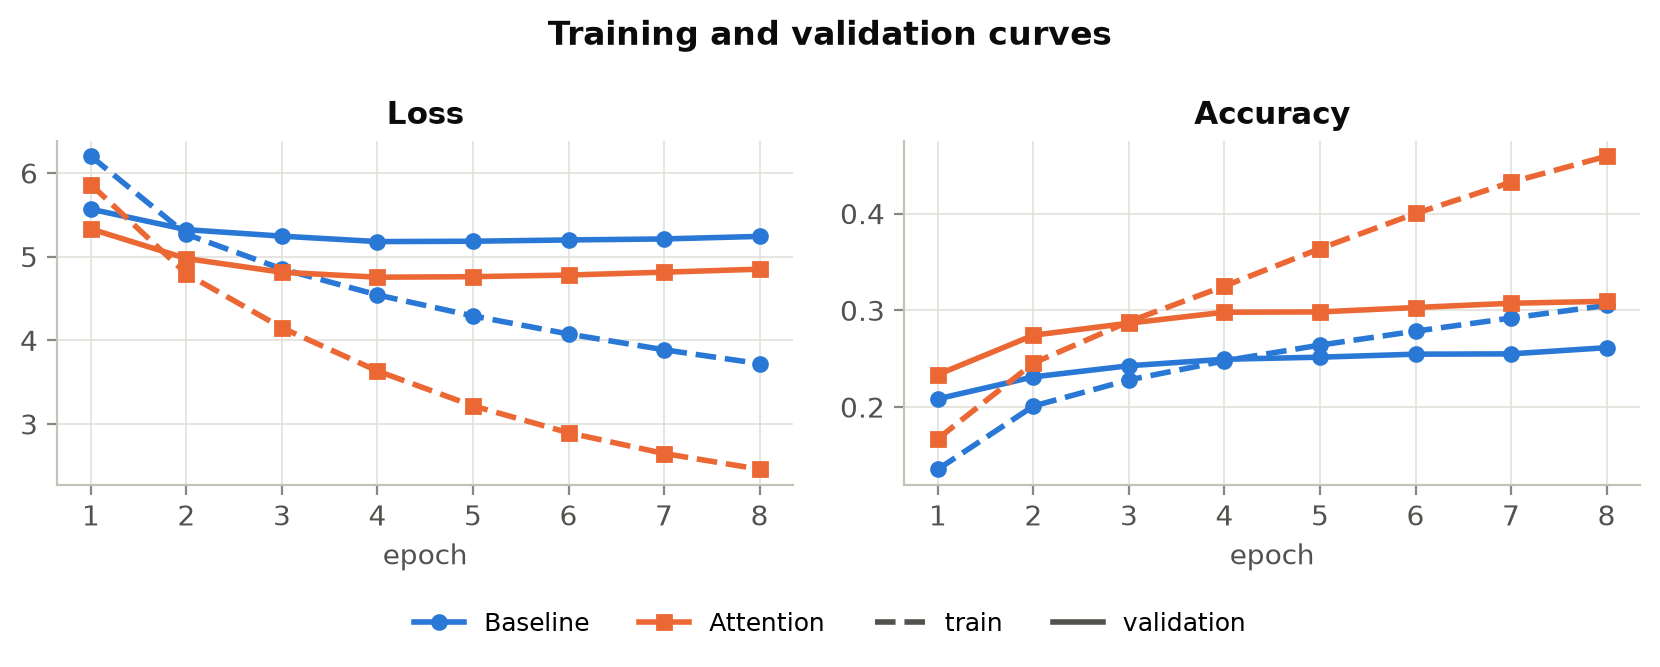
\includegraphics[width=\linewidth]{../outputs/figures/training_curves.png}
\caption{Training and validation loss (left) and token accuracy (right) for the baseline (A) and the attention model (B), seed 42. The best
epoch (4 for both) is the one with the lowest validation loss; that checkpoint is evaluated on the test set.}
\end{figure}

\begin{table}[H]\centering\small\tabHistory
\caption{Per-epoch values behind Figure 1 (loss is cross-entropy in nats; accuracy is masked next-token accuracy under teacher forcing). Bold:
epoch 4, the selected checkpoint. Early stopping ended both runs after epoch 8.}\end{table}

Both models overfit early: training loss keeps falling and training accuracy keeps rising (A reaches 0.305, B 0.459 at epoch 8), but validation
loss turns upward after epoch 4. With 50,000 pairs and 38--72M parameters this is expected. Attention is ahead of the baseline in
validation loss at every single epoch (for example 4.754 vs 5.180 at epoch 4) and fits the training data faster, but it also overfits more
strongly (train minus validation accuracy at epoch 8: 0.150 for B, 0.044 for A). Attention is also about 4.6 times slower per epoch (222 s vs 48 s
on an RTX 4050 laptop GPU).

%--------------------------------------------------------------------------------------------------------------
\section{Test-set results: all scores}
\begin{table}[H]\centering\tabMetrics\caption{Translation metrics on the full test set (2,393 sentences, greedy decoding). Bold = better model.
Precisions are in percent, BLEU is on a 0--100 scale.}\end{table}

\begin{table}[H]\centering\tabLoss\caption{Cross-entropy, accuracy and model size. Test loss and token accuracy are teacher-forced.}\end{table}

\textbf{Reading the numbers.} Attention wins on every metric. Unigram precision rises from 15.9\% to 24.0\%, so more of the generated words
appear in the reference; the higher-order precisions rise by a larger factor (bigram 2.2 $\rightarrow$ 5.3, trigram 0.19 $\rightarrow$ 1.13,
4-gram 0.01 $\rightarrow$ 0.21), which means attention produces some correct word sequences, whereas the baseline almost never does.
The brevity penalty is 1.0 for both (outputs are 3\% and 9\% longer than the references), so the BLEU gap is not a length artefact. TER above
100 for both models means a human would need more than one edit per reference word, i.e.\ neither system is close to usable translation;
the comparison is about \emph{relative} quality. Absolute BLEU stays low because (i) 50k pairs is about 3\% of the corpus, (ii) the vocabulary is
word-level with 8\% OOV, (iii) Hindi has free word order and rich morphology, which BLEU penalises with a single reference, and (iv) the training
mix and the news-style test set differ in domain. An earlier 30,000-pair run gave BLEU 0.02 (A) and 1.21 (B), the same ordering
(\code{outputs/results/archive\_run1\_30k/}).

%--------------------------------------------------------------------------------------------------------------
\section{Limitation of the baseline (Part 3)}
\textbf{Why long inputs are hard for Model A.} The decoder sees the source only through one 512-dimensional state. That vector has to hold
the content, word order and length of the whole sentence, so the longer the input, the more information is squeezed into the same size,
and the earliest words are the furthest from the point where the decoder starts. We tested three questions from the brief.

\textbf{Short vs long.} The test set was split into 1--5, 6--10, 11--15 and 16+ tokens (Table 5, and the full table in the Appendix).
\begin{table}[H]\centering\small\tabCompare\caption{Baseline (A) vs attention (B) by English sentence length. ``repeats'' is the share of outputs with a
repeated 3-gram.}\end{table}

\begin{itemize}
\item \textbf{We cannot show a clean decline of the baseline with length}, because its BLEU is already close to zero in every bucket with at
least 6 tokens (0.41, 0.48, 0.57). With nothing left to lose there is nothing to decline. Its chrF even rises with length (7.61 $\rightarrow$ 12.73), because long
sentences contain many frequent function words and punctuation that a content-blind model still matches.
\item \textbf{1--5 tokens:} A's BLEU (3.07) is higher than B's (2.13), but with 13 sentences this is not meaningful (and B's chrF, 12.77 vs
7.61, points the other way). Both models also produce outputs that are too short there (brevity penalties 0.786 and 0.688).
\item \textbf{Does the baseline use the source at all?} Its outputs for different inputs are close to generic Hindi sentences such as
\hi{एक दूसरे के साथ एक दूसरे से अधिक है}; unigram precision is only 15.9\%. We did not run a no-source ablation, so we cannot say exactly
how much of the baseline's output is conditioned on the input.
\item \textbf{Are early words lost?} We measured unigram recall of reference words by position in the reference for the 16+ bucket:
\end{itemize}
\begin{table}[H]\centering\tabRecall\caption{Recall of reference words by quarter of the reference sentence (16+ bucket, 1,617 sentences).}\end{table}
The baseline is poor everywhere and worst in the middle (0.13). The data do \emph{not} show a distinct ``beginning is forgotten'' effect: the last
quarter is best for both models, probably because it contains frequent closing words (\hi{है}, \hi{।}). Attention improves recall in every quarter,
by the largest margin at the start (0.165 $\rightarrow$ 0.275, 1.7$\times$).

\begin{figure}[H]\centering
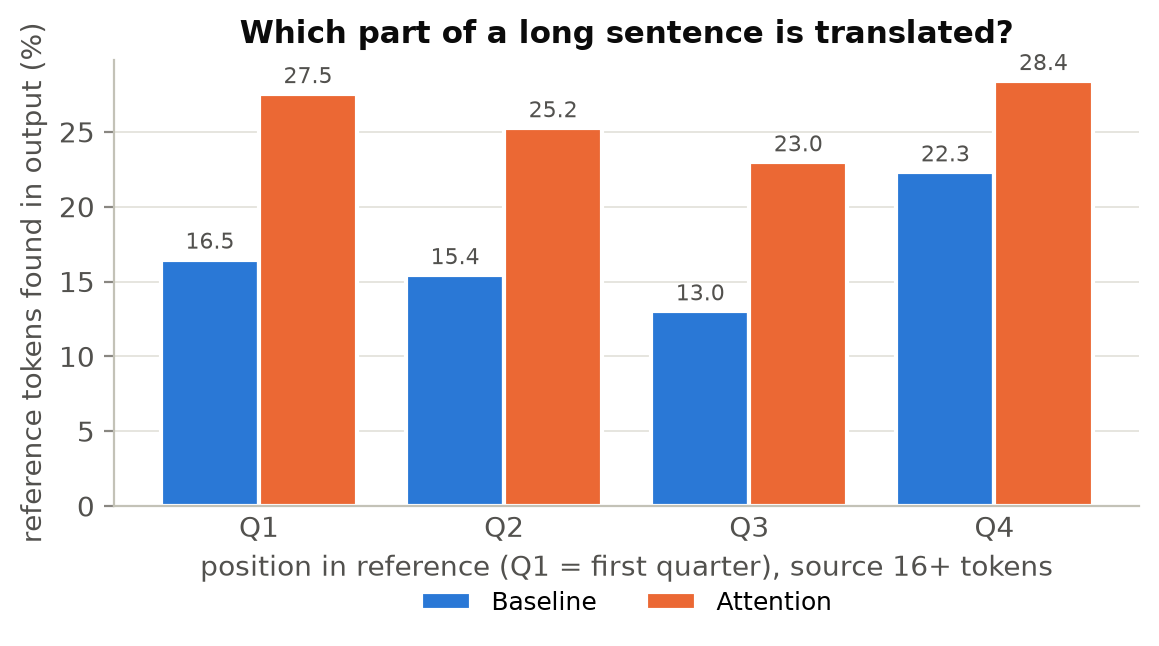
\includegraphics[width=0.56\linewidth]{../outputs/figures/position_recall.png}
\caption{Unigram recall of reference words by position in the reference sentence, 16+ bucket.}
\end{figure}

%--------------------------------------------------------------------------------------------------------------
\section{Performance by sentence length (Part 8)}
\begin{figure}[H]\centering
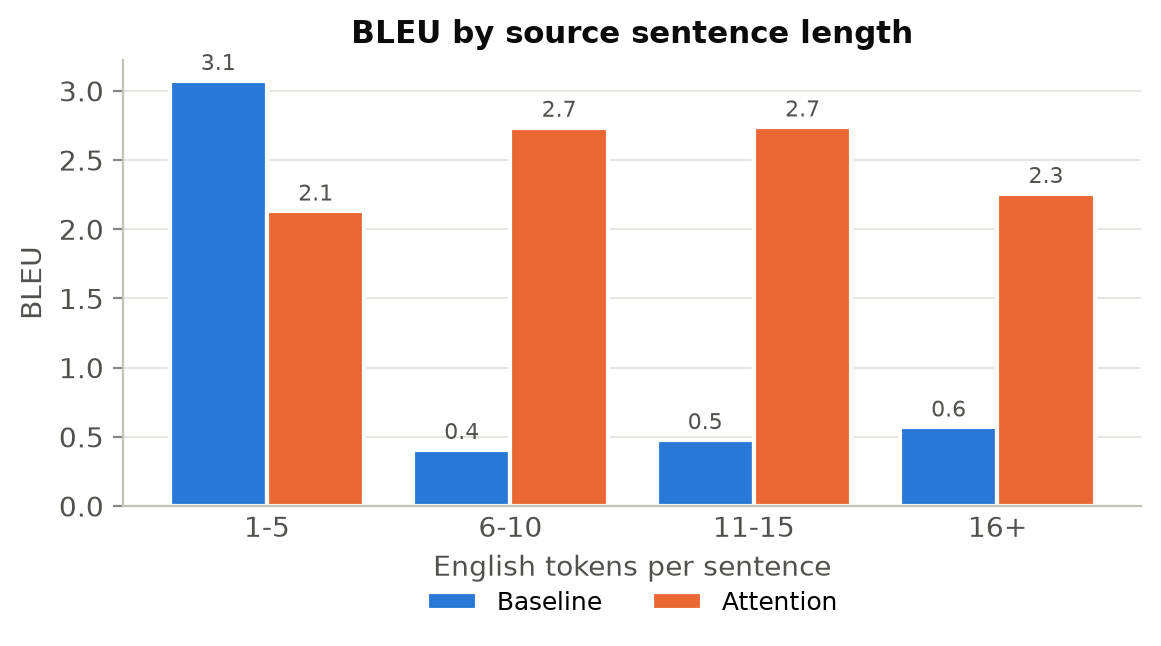
\includegraphics[width=0.92\linewidth]{../outputs/figures/length_analysis.png}
\caption{Test BLEU and chrF as a function of English sentence length, baseline (A) vs attention (B). Exact values are in Table 5 and the Appendix.}
\end{figure}
For sentences with 6 or more tokens the attention model is \textbf{4.0 to 6.8 times better in BLEU} (6--10: 0.41 vs 2.73, 6.8$\times$; 11--15: 0.48 vs
2.74, 5.7$\times$; 16+: 0.57 vs 2.26, 4.0$\times$) and consistently 5 to 7 chrF points better. B's BLEU is flat from 6--10 to 11--15 (2.73, 2.74)
and falls to 2.26 for 16+ while its chrF keeps rising (16.0, 17.1, 18.2); the baseline stays at the floor throughout. So the \emph{gap} narrows
slightly for the longest sentences in BLEU, but we cannot claim the baseline's decline with length is the cause, since it has nowhere to decline
to. A visible weakness of attention on long input is repetition: 17.6\% of its outputs for 16+ tokens contain a repeated 3-gram, against 0.5\% for the
baseline (Table 5). The 1--5 bucket (13 sentences) gives no usable comparison.

%--------------------------------------------------------------------------------------------------------------
\section{What the model attends to (Part 6)}
Each heatmap has the English tokens (with \sos{} and \eos{}) on the x-axis and the generated Hindi tokens on the y-axis; every row sums to 1.
Eleven examples spread across the length buckets are in \code{outputs/figures/attention\_heatmap\_01..11.png} (sentences and translations in
\code{heatmap\_examples.json}); four are shown here.

\begin{figure}[H]\centering
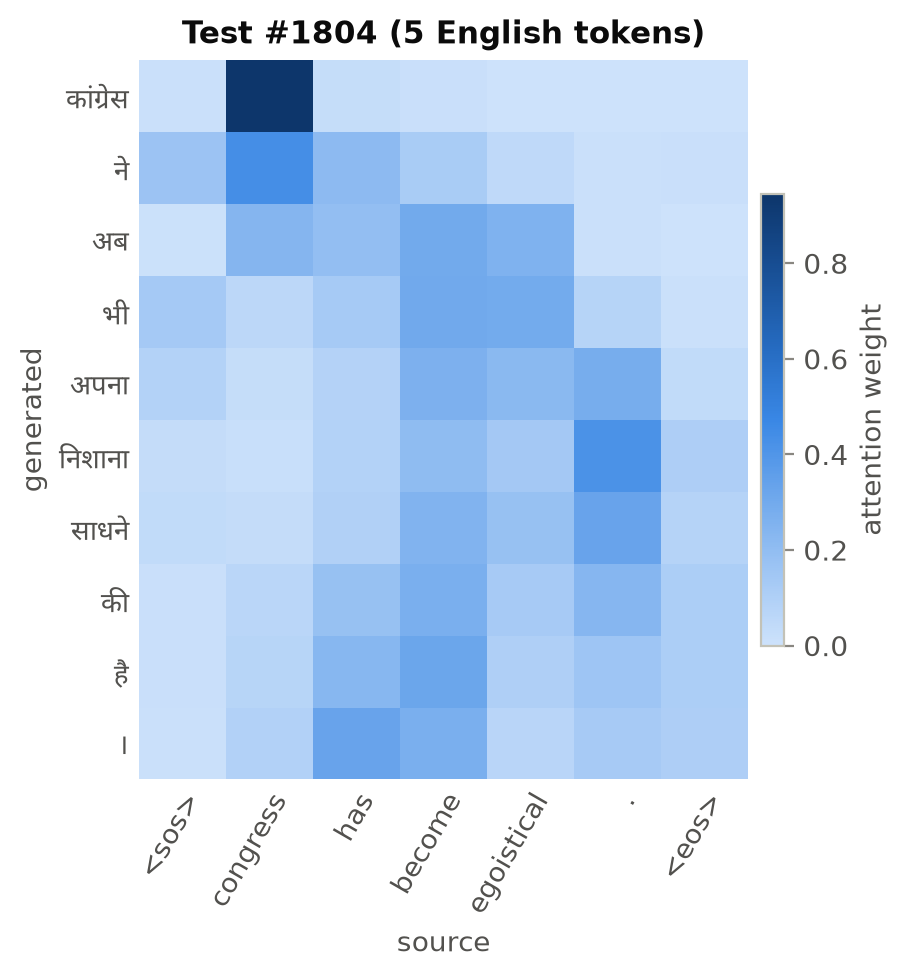
\includegraphics[width=0.49\linewidth,height=0.30\textheight]{../outputs/figures/attention_heatmap_01.png}\hfill
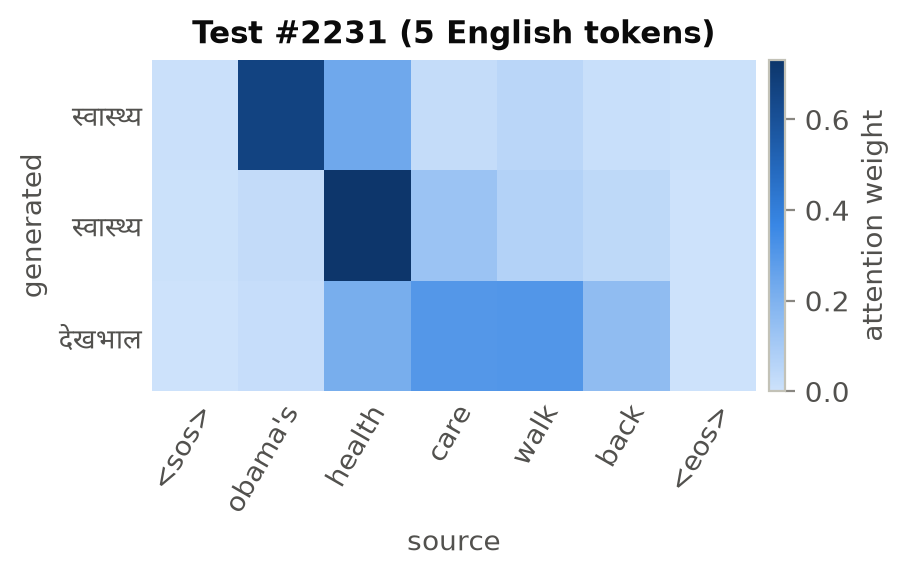
\includegraphics[width=0.49\linewidth,height=0.30\textheight]{../outputs/figures/attention_heatmap_02.png}\\[4pt]
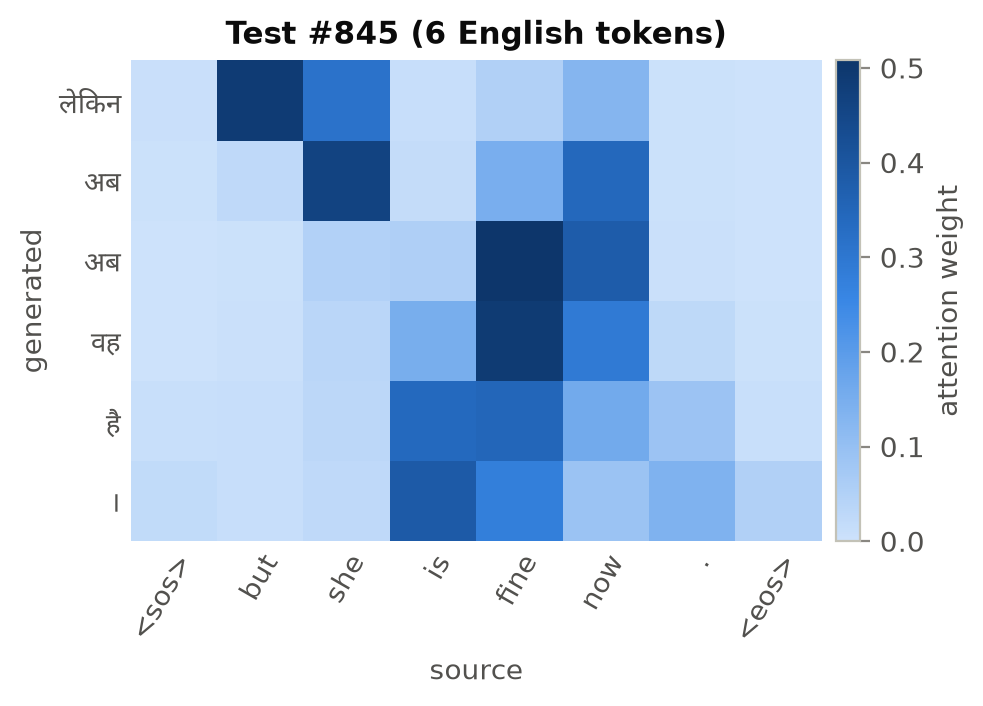
\includegraphics[width=0.49\linewidth,height=0.30\textheight]{../outputs/figures/attention_heatmap_04.png}\hfill
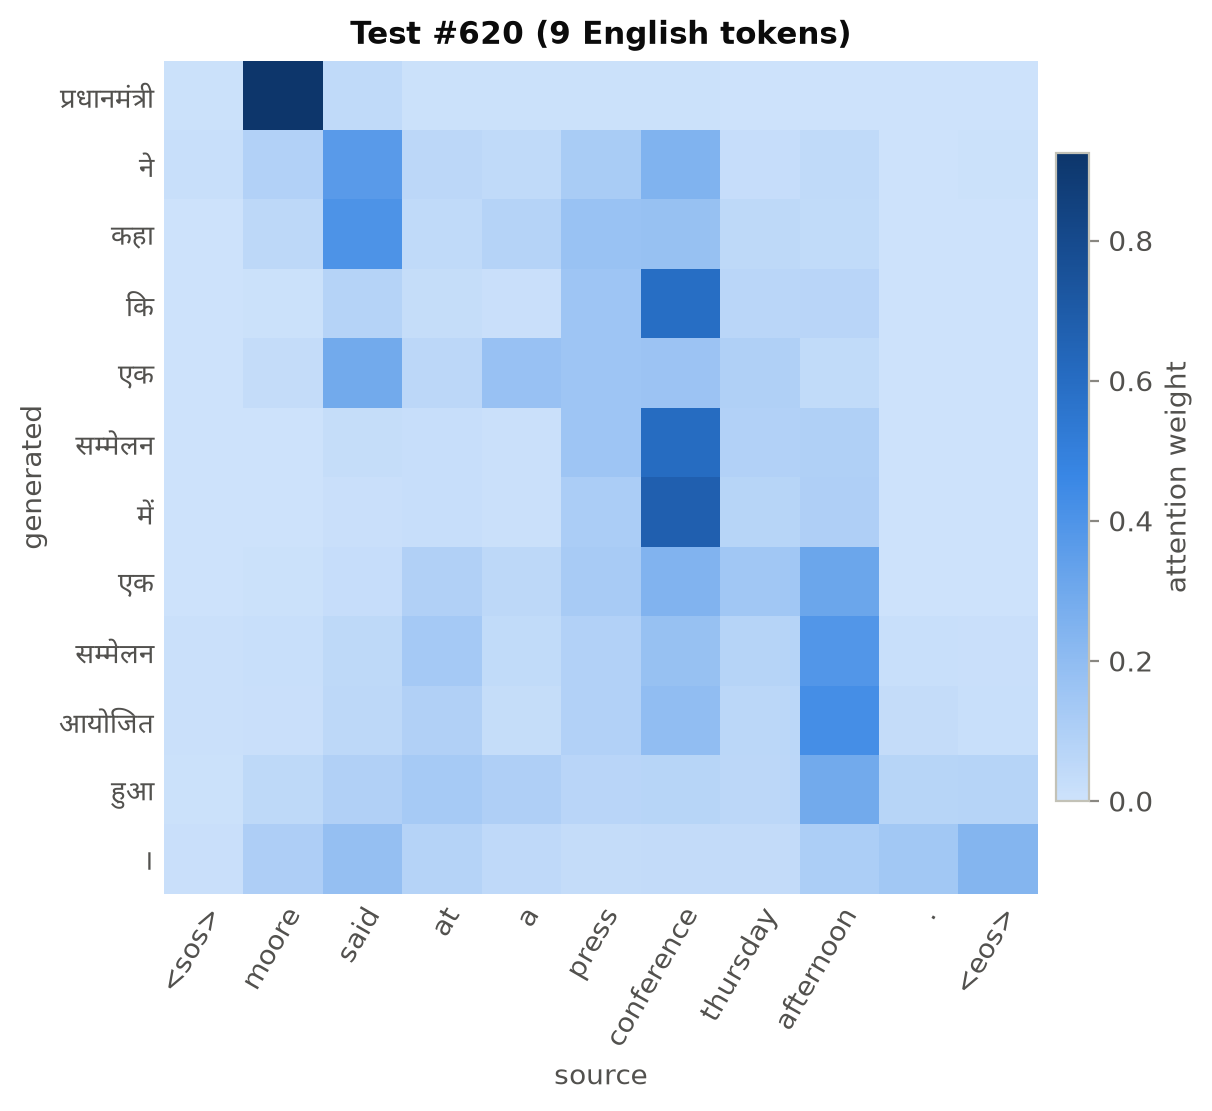
\includegraphics[width=0.49\linewidth,height=0.30\textheight]{../outputs/figures/attention_heatmap_05.png}
\caption{Attention heatmaps for test sentences 1804 (``congress has become egoistical .''), 2231, 845 and 620.}
\end{figure}

Statistics over \emph{all} 2,393 test sentences:
\begin{table}[H]\centering\tabAttn\caption{Attention statistics (\code{outputs/results/attention\_behaviour.json}).}\end{table}

\begin{itemize}
\item \textbf{Which English words get high attention?} Content words that have a one-to-one Hindi counterpart: \emph{congress} gets about 0.9 for
\hi{कांग्रेस}, \emph{both} about 0.85 for \hi{दोनों}.
\item \textbf{Does the model attend to the relevant word?} Often for content words, rarely for function words: the mean peak weight is only 0.277 and
the mean entropy is 2.32 nats, close to spreading weight over about 10 source tokens.
\item \textbf{Does attention move sequentially?} Mostly: in 85.3\% of steps the peak stays or moves forward. English is SVO and Hindi SOV, so verbs
and objects swap places, which shows as off-diagonal blocks (error case 5: \emph{sent} is attended at the end for \hi{भेजा गया है}).
\item \textbf{Multiple source words?} In 20.6\% of steps no word has weight 0.5 but two or more exceed 0.2, typically for phrases such as
\emph{would be used}, \emph{of the}, \emph{not only}.
\item \textbf{Incorrect attention?} Yes, in two ways: attention stuck on one column for many steps (case 1: \emph{university} for about 12 steps)
and attention anchored on punctuation (case 8: closing quote mark).
\item \textbf{Sinks.} \sos{}/\eos{} receive only 1.0\% of the attention mass, so the model does not use them as ``do nothing'' sinks.
\end{itemize}

%--------------------------------------------------------------------------------------------------------------
\section{Attention-based error analysis (Part 7)}
We selected \textbf{eight} test sentences where the attention model is wrong or partly wrong (sentence chrF between 22 and 55), picked to cover
different error types. For each: English input, reference, baseline output (A), attention output (B), the attention heatmap, an error
classification and a judgement of whether the heatmap explains the error. (Full table: \code{outputs/results/error\_cases.md}; cases are
numbered as in that file.)

\newcommand{\caseblock}[1]{\errorcase{#1}\par\vspace{2pt}
\begin{center}\includegraphics[width=0.86\linewidth,height=0.34\textheight]{../outputs/figures/error_case_0#1.png}\end{center}\vspace{-2pt}}

\subsection*{Cases 1 to 4}
\caseblock{1}\caseblock{2}
\caseblock{3}\caseblock{4}
\subsection*{Cases 5 to 8}
\caseblock{5}\caseblock{6}
\caseblock{7}\caseblock{8}

\subsection{Error types and what the heatmap tells us}
\begin{enumerate}
\item \textbf{OOV words} (names and acronyms: 8\% of test tokens) are the largest single cause: dropped or replaced by generic words in 7 of 8
cases (\emph{tassie}, \emph{bcci}, \emph{mca}, \emph{amarnath upadhyaya}, \emph{nita}, \emph{isha}). Attention cannot translate a word that is not in the output vocabulary;
a copy mechanism or subword units would be needed.
\item \textbf{Repetition} appears in 5 of 8 cases and in 17.6\% of long outputs. The decoder is given more to say but nothing stops it saying the
same thing twice (no coverage mechanism).
\item \textbf{Long-distance dependency.} In cases 1, 7 and 8 the first half is translated sensibly and the diagonal breaks in the second half.
\item \textbf{Right focus, wrong word} (cases 2, 3, 4, 6): attention sits on the correct source words but the decoder's lexical choice fails, a
vocabulary and data-size problem rather than an alignment problem.
\item \textbf{Is the heatmap a useful explanation?} It is useful for \emph{locating} a failure (the stuck column in case 1, the broken diagonal in
case 7, punctuation anchoring in case 8) and for confirming that content words are aligned. It is not a guarantee of correctness: in cases 4 and 6
the heatmap looks like a good translation of a wrong sentence, and the baseline has no heatmap at all, so its errors cannot be inspected this way.
\end{enumerate}

%--------------------------------------------------------------------------------------------------------------
\section{Final comparative analysis (Part 9)}
\begin{itemize}
\item \textbf{How does attention compare with the baseline?} Clearly better on every measure from one seed: BLEU 0.55 $\rightarrow$ 2.34 (4.3$\times$), chrF 12.27 $\rightarrow$ 17.91,
chrF++ 11.54 $\rightarrow$ 17.37, TER 104.0 $\rightarrow$ 99.1, validation loss 5.18 $\rightarrow$ 4.75, test perplexity 160 $\rightarrow$ 106, token accuracy 0.243 $\rightarrow$ 0.290.
\item \textbf{Short or long sentences?} For 6+ tokens attention is 4.0--6.8$\times$ better in BLEU, with the largest ratio at 6--10 tokens; its BLEU is
flat at about 2.7 for 6--15 and 2.26 for 16+, while the baseline is at the floor in every bucket. On the 13 sentences with 1--5 tokens the result is inconclusive.
\item \textbf{Which errors were reduced?} The baseline's fully generic, source-independent outputs are largely gone. Attention outputs contain the topic
words (\hi{बाजार}, \hi{केंद्रीय}, \hi{सरकार}, \hi{भेजा गया}), keep correct sentence openings (\hi{इसके अलावा}) and align many content words.
\item \textbf{Which errors remain or got worse?} OOV words, long-distance structure, and repetition (17.6\% of long outputs vs 0.5\%).
\item \textbf{What do the heatmaps reveal?} Mostly forward-moving alignment, sharp on single content words, diffuse on function words and long phrases;
failures appear as a stuck column or attention on punctuation.
\item \textbf{Do high attention weights always mean a correct translation?} No. The mean peak weight is 0.2769 for generated tokens that occur in
the reference and 0.2768 for those that do not, i.e.\ identical. In case 4, \emph{abroad} gets weight about 0.65 three steps in a row and the model writes
\hi{भी भी भी}.
\item \textbf{Can attention be used as an explanation?} Partly. It is a reliable \emph{diagnostic of where the model looked} and helps locate
alignment breakdowns, but weights do not separate right words from wrong ones, so it should not be read as proof of why a word was produced or whether it is correct.
\end{itemize}

\subsection*{Limitations}
\begin{itemize}
\item One seed per model and no confidence intervals; a difference of the size we see is large, but we cannot quantify run-to-run variance.
\item Low absolute scores: 50,000 training pairs, word-level vocabulary without subwords (8\% OOV), single reference, greedy decoding only (no beam search).
\item Model B has almost twice the parameters of Model A (71.9M vs 38.3M), so part of the gain may come from capacity rather than attention alone.
\item The test set is 68\% long sentences and the 1--5 bucket has 13 sentences, so short-sentence conclusions are weak.
\item Error types in section 9 were assigned by hand to eight sentences and are illustrative, not a statistical sample (the aggregate statistics in
sections 7 and 8 cover all 2,393 sentences).
\item Banning \unk{} during decoding is a pragmatic fix; it applies to both models but means OOV words are replaced rather than flagged.
\end{itemize}

%--------------------------------------------------------------------------------------------------------------
\section{Where every score is stored and how to reproduce it}
\textbf{All evaluation scores are written out in full in} the files \code{all\_evaluation\_scores.md}, \code{.csv} and \code{.json} in \code{Question-1/outputs/results/}, generated by
\code{Question-1/scores\_report.py}. That script recomputes every metric from the saved test predictions and checks that BLEU and chrF match the
values saved by \code{evaluate.py} (they do, to $10^{-6}$).

\begin{table}[H]\centering\small
\begin{tabular}{@{}p{0.43\linewidth}p{0.5\linewidth}@{}}\toprule
File (under \code{Question-1/outputs/results/}) & Contents\\\midrule
\code{all\_evaluation\_scores.*} & every metric above, overall and per length bucket, both models\\
\code{*\_seed42/test\_bleu.json} & BLEU, chrF, precisions, brevity penalty, lengths, test loss, token accuracy\\
\code{*\_seed42/bucket\_bleu.json, bucket\_stats.json} & BLEU and chrF per length bucket (with n, BP, length ratio)\\
\code{*\_seed42/history.json} & per-epoch train/validation loss and accuracy, time\\
\code{*\_seed42/test\_predictions.jsonl} & source, reference and output for each of the 2,393 test sentences\\
\code{baseline\_limitation.json} & length-bucket repetition, length ratio, position recall\\
\code{attention\_behaviour.json} & attention statistics (Table 7)\\
\code{error\_cases.md/json, error\_case\_notes.json} & the eight error cases and our notes\\
\code{comparison\_tables.md, model\_comparison.json} & summary tables\\\bottomrule
\end{tabular}\caption{Result files.}\end{table}

\begin{verbatim}
pip install -e ".[dev]" && pip install -r Question-1/requirements.txt
cd Question-1
python train.py --model both --epochs 20 --patience 4
python evaluate.py                                      # test metrics, predictions
python analysis.py                                      # limitation, attention stats, errors
python visualize.py                                     # curves, heatmaps
python scores_report.py                                 # all scores in one table
python report/make_tables.py && (cd report && xelatex Q1_report.tex && xelatex Q1_report.tex)
\end{verbatim}

%--------------------------------------------------------------------------------------------------------------
\appendix
\section{Appendix: complete scores by sentence length}
\begin{table}[H]\centering\small\tabBucketA\caption{Model A (baseline), all metrics per English-length bucket. p1--p4 are BLEU n-gram precisions in percent,
BP the brevity penalty, ratio the hypothesis/reference token ratio.}\end{table}
\begin{table}[H]\centering\small\tabBucketB\caption{Model B (attention), same columns.}\end{table}
The brevity penalty below 1 for 1--5 and 6--10 tokens shows that both models under-generate for short inputs; for 11+ tokens the outputs are longer
than the references (ratio 1.02--1.12), which is where repetition appears.

\end{document}
